\section{Verstärkendes Lernen}
Verstärkendes Lernen oder als RL in der Fachsprache bezeichnet, definiert einen konzeptionellen Ansatz zielorientiertes Lernen von Entscheidungen zu verstehen und zu automatisieren. \footcite[Vgl.][S. 13]{Sutton.2018}
Dabei besteht der Fokus darauf, dass ein Agent aus der direkten Interaktion mit seiner Umgebung lernt, ohne das explizite Überwachung notwendig ist. \footcite[Vgl.][S. 13]{Sutton.2018}
Der Agent lernt über die Zeit eine optimale Strategie zur Lösung des Entscheidungsproblems aus dem Ausprobieren und Scheitern mittels verschiedener Aktionen die gewünschte Veränderung in seiner Umwelt herzustellen. \footcite[Vgl.][S. 4]{Li.2019}
Notwendig dabei ist es, dass der Agent den Zustand seiner Umgebung wahrnehmen, und auch durch entsprechende Aktionen beeinflussen kann, sodass die Erreichung des Zielzustandes möglich ist. \footcite[Vgl.][S. 2]{Sutton.2018}
Zur Erreichung dieses Zielzustandes muss der Agent alle Aktionen entdecken, welche ihm die größtmögliche kumulierte Belohnung liefern, wobei Aktionen nicht nur die unmittelbare sondern auch zukünftige Belohnungen beeinflussen. \footcite[Vgl.][S. 1]{Sutton.2018}
%Damit grenzt RL sich vom überwachten Lernen in der Art und Weise ab, dass dem Agenten zwar evaluiertes Feedback zur Verfügung steht, jedoch keine direkte Kennzeichnung ob seine Aktion korrekt oder falsch war.\footcite[Vgl.][S. 4]{Li.2019} 
Zusammengefasst lässt sich die beschriebene Interaktion des Agenten mit seiner Umgebung wie folgt in Abbildung 1 darstellen.
\begin{figure}[htb]
    \centering
    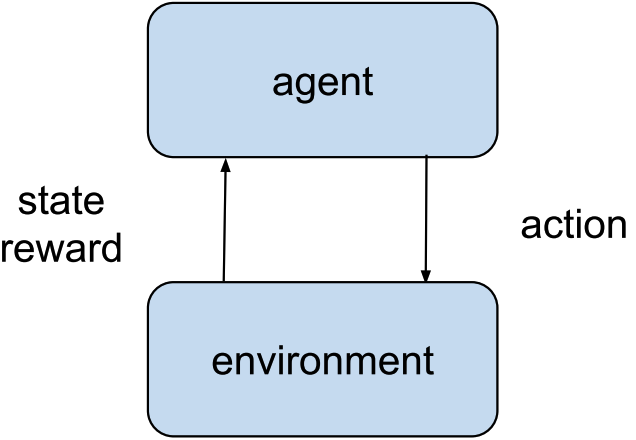
\includegraphics[height=4cm]{lib/graphics/Agent-Environment interaction.png}
    \caption[vereinfachte Darstellung der Interaktion zwischen dem Agenten und seiner Umgebung]{vereinfachte Darstellung der Interaktion zwischen dem Agenten und seiner Umgebung\footnotemark}
    \label{abb:Agent-Environment interaction}
\end{figure}
\footnotetext{Enthalten in: \cite[][S. 5]{Li.2019}}

Ein Standardaufbau einer Aufgabe für verstärkendes Lernen kann demnach verstanden werden, als sequentielles Entscheidungsproblem zu dessen Lösung ein Agent zu jedem diskreten Zeitschritt eine Aktion ausführt, welche den Zustand der Umgebung verändert. \footcite[Vgl.][S. 2]{Zhao.2020}
Betrachtet man die technische Umsetzung einer solchen Interaktion zwischen dem Agenten und dessen Umgebung, wird häufig zur Modellierung ein Markov Entscheidungsprozess verwendet.
Im Kontext von RL ist der Entscheidungsprozess definiert nach einem Tupel aus folgenden Elementen:\footcite[Vgl.][S. 2]{Zhang.2018}
\begin{itemize}
    \item Alle Zustände $S$
    \item Alle Aktionen $A$
    \item initiale Zustandsverteilung $p0(S)$
    \item Übergangswahrscheinlichkeit $T(S_{t+1}|S_{t},A_{t})$
    \item Belohnungswahrscheinlichkeit $R(r_{t+1}|S_{t},A_{t})$
\end{itemize}

Zum Finden der optimalen Strategie existieren modellbasierende und modellfreie Algorithmen des verstärkenden Lernens. \footcite[Vgl.][S. 3]{Wang.2020}
Bei modellbasierenden Algorithmen wird das Umgebungsverhalten, also die Übergangs- und Belohnungswahrscheinlichkeiten als bekannt vorausgesetzt. \footcite[Vgl.][S. 3]{Wang.2020}
Unter modellbasierenden Algorithmen wird dynamische Programmierung eingesetzt, um mittels Strategieevaluation und Strategieiteration die optimale Strategie zu finden. \footcite[Vgl.][S. 5]{Li.2019}
Unter modellfreien Algorithmen werden die drei verschiedenen Ansätze Wertebasierend, Strategiebasierend und Akteur-Kritiker basierend unterschieden \footcite[Vgl.][S. 5]{Li.2019}
Der Agent im Kontext von modellfreien RL Methoden kennt nur die Zustände $S$ und die Aktionen $A$, jedoch nicht die Umgebungsverhalten $T$ und die Belohnungswahrscheinlichkeit $R$. \footcite[Vgl.][S. 2]{Cutler.2014}
%Im Kontext von modellbasierendem RL im Vergleich zum modellfreien RL sind die Übergangs- und Belohnungswahrscheinlichkeiten bekannt, wodurch mittels Strategie- und Werteevaluation sowie Optimierung die bestmögliche Strategie gefunden werden kann. \footcite[Vgl.][S. 5]{Li.2019}
Fasst man die Klassifizierung der Algorithmen und Methoden von RL zusammen, lässt sie sich wie folgt darstellen:

\begin{figure}[htb]
    \centering
    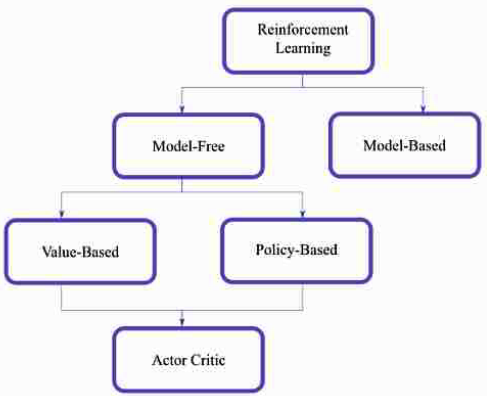
\includegraphics[height=5cm]{lib/graphics/taxonomy of RL algorithms.png}
    \caption[Klassifizierung von Algorithmen im Bereich des RL]{Klassifizierung von Algorithmen im Bereich des RL\footnotemark}
    \label{abb:RL-algorithm-classification}
\end{figure}
\footnotetext{Enthalten in: \cite[][S. 6]{Canese.2021}}

\subsection{Methoden des verstärkenden Lernens}
%\subsection{Wertebasierende Methoden}
Der Agent sucht in diesem Kontext die optimale Strategie $\pi^{*}$, welche allen Zuständen $S$ die jeweilige Aktion $A(S)$ zuordnet, sodass die kummulierte Belohnungswahrscheinlichkeit $R(r_{t+1}|S_{t},A_{t})$ über alle Zeitschritte $t$ maximal ist. \footcite[Vgl.][S. 2]{Reda.2020}
Neben dieser kurzfristigen direkten Belohnung müssen auch die langfristigen zukünftigen Belohnungen aus den neuen Zuständen betrachtet werden, wofür das Konzept der Wertigkeit eingeführt wird. \footcite[Vgl.][S. 3]{Wang.2020}
Über eine Zustands- oder Aktionswertigkeitsfunktion, oftmals als Q-Funktion referenziert, wird eine Vorhersage über die zu erwartende kumulierte abgezinste zukünftige Belohnung berechnet.\footcite[Vgl.][S. 5]{Li.2019}
Durch den Abzinsungsfaktor $\gamma \in \left[0,1\right)$ wird der Einfluss zukünftiger Belohnungen nach ihrer zeitlichen Reihenfolge priorisiert.\footcite[Vgl][S. 5]{Li.2019}
Mit der Wertigkeitsfunktion kann evaluiert werden, welche Strategie langfristig am erfolgreichsten ist, da bspw. manche Aktionen trotz geringer sofortiger Belohnung einen hohen Wert aufweisen können, wenn aus dem zukünftigen Zustand eine hohe Belohnung zu erwarten ist.\footcite[Vgl.][S. 6]{Sutton.2018}
Die Wertigkeitsfunktion und die daraus berechneten Wertigkeiten von Aktionen oder Zuständen werden über alle Zeitschritte neu geschätzt und stellen mit die wichtigste Komponenten in Algorithmen des verstärkenden Lernens dar. \footcite[Vgl.][S. 6f.]{Sutton.2018}
Methoden basierend auf diesem Wertigkeitswert lernen eine Schätzfunktion der Wertigkeit für alle Zustände ($V_{\pi}(s) \forall S$) und alle Zustandsaktions-Paare ($Q_{\pi}(s_{t},a_{t}) \forall s,a \in (S,A)$) der optimalen Strategie $\pi^{*}$ durch aktualisieren der folgenden Funktionen eins und zwei: \footcite[Vgl.][S. 2]{Zhang.2018}
\begin{description}
    %\item 1: $Q(s_{t}, a_{t}| \omega_{t+1}) \leftarrow Q(s_{t}, a_{t}|\omega_{t}) + \alpha\left[r_{t+1} + \gamma\max\limits_{a}Q(s_{t+1},a|\omega)-Q(s_{t},a_{t}|\omega)\right]*\nabla_{\omega}Q(s_{t},a_{t}|\omega)$
    \item \begin{center} (1) $Q(s_{t}, a_{t}) \leftarrow Q(s_{t}, a_{t}) + \alpha\left[r_{t+1} + \gamma\max\limits_{a}Q(s_{t+1},a)-Q(s_{t},a_{t})\right]$ \end{center}
    \item \begin{center} (2) $V(s_{t}) = \max\limits_{a}Q(s_{t},a|\omega)$ \end{center}
\end{description}
Aus den geschätzten Wertigkeit jedes Zustandsaktions Paares kann die optimale Strategie $\pi^{*}(s)$ durch $\underset{a}{\arg\max}$ $Q(s,a)$ bestimmt werden. \footcite[Vgl.][S. 2]{Zhang.2018}

%\subsection{Strategiebasierende Methoden}
Methoden, welche die Strategie durch deren direkte Parametrisierung anstelle einer Bewertung aller Handlungsalternativen mittels Wertigkeitsfunktion optimieren, werden als strategiebasierend bezeichnet. \footcite[Vgl.][S. 2]{Zhang.2018}
Diese Methodik kann beim Trainieren deterministischer Strategien zu unerwarteten Aktionen führen, weshalb häufig das Optimieren einer Wahrscheinlichkeitsverteilung für alle Aktionen bevorzugt wird. \footcite[Vgl.][S. 3]{Ningombam.2022}
Als Subklasse der RL Methoden wird der statistische Gradientenabstieg verwendet um die parametrisierte Strategie $\pi_{\theta}$ hinsichtlich der maximalen langfristigen kumulierten Belohnung zu optimieren. \footcite[Vgl.][S. 3]{Ningombam.2022}
Die Strategie $\pi_{\theta}$ oder auch $\pi(a|s,\theta)$ beschreibt dabei die Wahrscheinlichkeit Aktion $a$ im Zustand $s$ auszuwählen unter dem Parametervektor $\theta$. \footcite[Vgl.][S. 321]{Sutton.2018}
Zur Optimierung der Strategie wird die Funktion der kumulierten Belohnungen $J$ nach dem Parameter der Gewichte $\theta$ wie folgt in Formel drei abgeleitet und der optimierte Parametervektor anhand Formel vier aktualisiert. \footcite[Vgl.][S. 6]{Wang.2020}
\begin{description}
    \item \begin{center} (3) $\nabla_{\theta}J(\theta) \approx \frac{1}{N} \sum \limits_{i=1}^{N} \left[(\sum \limits_{t=1}^{T} \nabla_{\theta}\log\pi_{\theta}(a_{t}|s_{t}))(\sum \limits_{t=1}^{T} r(s_{t},a_{t}))\right]$ \end{center}
    \item \begin{center} (4) $\theta \leftarrow \theta + \alpha\nabla_{\theta}J(\theta)$ \end{center}
\end{description}
Zusammengefasst kann Formel vier und fünf dabei so interpretiert werden, dass die logarithmierte Wahrscheinlichkeit Aktion $a_{t}$ im Zustand $s_{t}$ auszuwählen erhöht werden soll, wenn $a_{t}$ in einer höheren kumulierten Belohnung resultiert. \footcite[Vgl.][S. 6]{Wang.2020}

%\subsection{Akteur-Kritiker Methoden}
Unter Akteur-Kritiker Methoden werden hybride wertebasierende und strategiebasierende Methoden verstanden, welche zugleich die Strategie optimieren und eine Wertefunktion approximieren. \footcite[Vgl.][S. 2f.]{Zhang.2018}
Die strategiebasierende Methodik mit der lernenden Strategie agiert dabei als Akteur, wohingegen die Wertefunktion, welche jeder Aktion und jedem Zustand einen Behlohnungswert zuweist, als Kritiker handelt. \footcite[Vgl.][S. 321]{Sutton.2018}
Der Akteur wählt somit aus seiner Wahrscheinlichkeitsverteilung die auszuführende Aktionen aus, während der Kritiker diese anhand seiner Wertigkeit bewertet. \footcite[Vgl.][S. 3]{Ningombam.2022}
Betrachtet man den Trainingsprozess von Akteur-Kritiker basierten Methoden ist dieser wie folgt aufgebaut: \footcite[Vgl.][S. 4]{Ningombam.2022}
\begin{itemize}
    \item Aktueller Zustand der Umgebung als Eingabe dem Akteur und Kritiker übergeben
    \item Akteur liefert eine auszuführende Aktion basierend auf dem Umgebungszustand
    \item Der Kritiker bekommt die Aktion als Eingabe und berechnet dessen Wertigkeit mittels Q-Funktion
    \item Durch die Wertigkeit seiner Aktion kann der Akteur seine Strategie anpassen
    \item Mit der neuen Strategie führt der Akteur die nächste Aktion im folgenden Zustand aus
    \item Die Q-Funktion des Kritikers wird mit den neuen Informationen aus der erhaltenen Belohnung angepasst
\end{itemize}

\subsection{Algorithmen des verstärkenden Lernens}

\subsection{Abgrenzung zu Multi-Agent Reinforcement Learning (MARL) Algorithmen}
Innerhalb dieses Unterkapitels soll der beschriebene Aufbau von RL Algorithmen und deren Optimierungsproblem zu den von MARL Systemen abgegrenzt werden.
Bei MARL Systemen wird anstatt einem Agenten eine Menge von Agenten eingesetzt welche alle mit ihrer Umgebung interagieren um den Weg der Zielerreichung zu lernen. \footcite[Vgl.][S. 6]{Wong.2022}
Dieser Ansatz dient dazu Problemstellungen welche nicht vollständig durch einen Agenten lösbar sind zu bearbeiten. \footcite[Vgl.][S. 1]{Canese.2021}
Einsatzgebiete von MARL sind dabei unter anderem das Routing von Netzwerkpaketen, Wirtschaftsmodellierung oder zusammenhängende Robotersysteme. \footcite[Vgl.][S. 1]{Canese.2021}
Je nach Ziel und der demnach definierter Belohnungsfunktion können die Agenten auf die drei unterschiedlichen Arten vollständig kooperativ, vollständig kompetitiv und der Mischung aus beiden miteinander interagieren. \footcite[Vgl.][S. 8f.]{Canese.2021}
Aus der unterschiedlichen Interaktion jedes Agenten mit der selben Umgebung ergibt sich der Unterschied, dass die Umgebungsdynamik aus der Kombination aller Aktionen der Agenten beeinflusst wird anstatt aus der Aktion des einzelnen Agenten. \footcite[Vgl.][S. 2]{Wong.2022}
Da dieser Effekt auch die Annahme der Stationarität von Markov Entscheidungsprozessen verletzt, bedarf dieUmgebung  auch einer anderen Representation. \footcite[Vgl.][S. 6]{Wong.2022}
Ein Konzept was dafür häufig verwendet ist das Markov Spiel, welches sich anders als der Entscheidungsprozess durch einen mehrdimensionalen Aktions- und Belohnungsraum aus der Kombination aller $N$ Agenten auszeichnet. \footcite[Vgl.][S. 4]{Canese.2021}
Betrachtet man die Limitierungen von MARL erkennt man aus den beschriebenen Punkten die Herausforderungen der nicht vorhandenen Stationarität und der Skalierbarkeit, welcher sich die Herausforderung der teilweisen Beobachtbarkeit der Umgebung anschließt. \footcite[Vgl.][S. 9ff.]{Canese.2021}

\subsection{Limitierungen und Herausforderungen von RL}
%Ein vorteilhafter Kernanspekt von RL ist die vollständige Betrachtung des Problems eines Zielgerichteten Agenten in einer unsicheren Umgebung. \footcite[Vgl.][S. 3]{Sutton.2018}
Trotz signifikanter Errungenschaften birgt der Einsatz von den besprochenen RL Algorithmen weiterhin Limitierungen und Risiken für ungewolltes Verhalten. \footcite[Vgl.][S. 7]{Li.2019}

Eine der Herausforderungen zeigt sich bei der Representation der Agentenumwelt, da RL stark auf diesem Konzept basiert. \footcite[Vgl.][S. 8]{Sutton.2018}
Daraus ergibt sich die Aufgabe, die Umwelt und dessen Verhalten sowie die Wahrnehmung durch den Agenten realitätsgetreu und präzise zu gestalten. \footcite[Vgl.][S. 7]{Sutton.2018}
Neben der Definition und Wahrnehmung des Umweltverhaltens ist die Spezifikation des Ziels des Agenten ein ebenso kritischer Teil, da unerwartete Intentionen aus der Zielstellung abgeleitet werden könnten. \footcite[Vgl.][S. 7]{Li.2019}
Zusätzlich teilen RL Algorithmen auch Herausforderungen aus anderen Gebieten des maschinellen Lernens wie Genauigkeit, Interpretierbarkeit und die im Rahmen dieser Arbeit untersuchte Robustheit von Modellen. \footcite[Vgl.][S. 7]{Li.2019}

Eine weitere Limitierung stellt der große Suchraum an Aktionen und das unbekannte Verhalten der Umgebung dar.
Dies sorgt dafür, dass häufig die Effizienz einzelner Daten sehr gering ist und die Abwägung zwischen Exploration neuer Strategie und der Optimierung bekannter Verhaltensmuster ein wichtiger Bestandteil ist. \footcite[Vgl.][S. 7]{Li.2019}
Aufgrund der geringen Effizienz der Daten aber des dennoch hohen Bedarfs an bewerteter Agentenerfahrung wird häufig auf simulierte Daten zurückgegriffen. \footcite[Vgl.][S. 7]{Zhao.2020}
Simulierte Daten werden dabei häufig von möglichst hoch qualitativen Simulationsumgebungen bereitgestellt, da zu dem hohen Bedarf der Methodik häufig Limitierungen in der Sammlung von Daten in der echten Welt bestehen. \footcite[Vgl.][S. 8]{Li.2019}

Aufgrund dieser Bedeutung der Simulationsumgebung für RL Algorithmen und deren Transfer in die echte Welt werden im nachfolgenden Kapitel die Merkmale und Entwicklungen von Simulationen genauer betrachtet.